\documentclass[test.tex]{subfiles}
\begin{document}

To jest teks rozdziału pierwszego \cite{Nowak} . Piszę w nim o dupie maryni.
Lorem ipsum tralkala. To jest teks rozdziału pierwszego. Piszę w nim o dupie maryni.
Lorem ipsum tralkala. To jest teks rozdziału pierwszego. Piszę w nim o dupie maryni.
Lorem ipsum tralkala. 



To jest teks rozdziału pierwszego. Piszę w nim o dupie maryni.
Lorem ipsum tralkala. To jest teks rozdziału pierwszego. Piszę w nim o dupie maryni.
Lorem ipsum tralkala. 
To jest teks rozdziału pierwszego. Piszę w nim o dupie maryni.
Lorem ipsum tralkala. To jest teks rozdziału pierwszego. Piszę w nim o dupie maryni.
Lorem ipsum tralkala.  

\newpage
\begin{figure}[h]
\centering
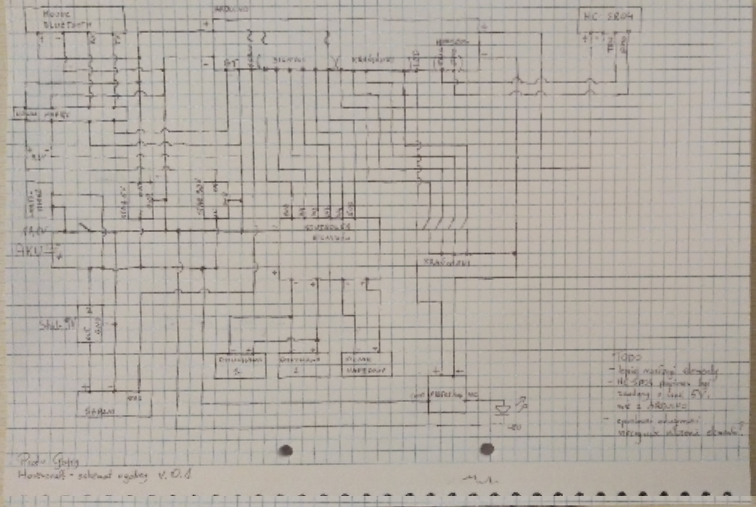
\includegraphics[width=1\textwidth]{./obrazy/R1/schemat_v01.jpg}
\caption{Wstępny schemat}
\label{image-myimage}
\end{figure}

Teraz pojawi się wzór!
$$1+2=3$$

A teraz numerowany wzór:
\begin{equation}
2^{2-a}=4_{E}
\end{equation}
Ułamki:$$\frac{A^C}{V_g}$$


\end{document}
